% Options for packages loaded elsewhere
\PassOptionsToPackage{unicode}{hyperref}
\PassOptionsToPackage{hyphens}{url}
%
\documentclass[
  english,
  man]{apa6}
\usepackage{lmodern}
\usepackage{amsmath}
\usepackage{ifxetex,ifluatex}
\ifnum 0\ifxetex 1\fi\ifluatex 1\fi=0 % if pdftex
  \usepackage[T1]{fontenc}
  \usepackage[utf8]{inputenc}
  \usepackage{textcomp} % provide euro and other symbols
  \usepackage{amssymb}
\else % if luatex or xetex
  \usepackage{unicode-math}
  \defaultfontfeatures{Scale=MatchLowercase}
  \defaultfontfeatures[\rmfamily]{Ligatures=TeX,Scale=1}
\fi
% Use upquote if available, for straight quotes in verbatim environments
\IfFileExists{upquote.sty}{\usepackage{upquote}}{}
\IfFileExists{microtype.sty}{% use microtype if available
  \usepackage[]{microtype}
  \UseMicrotypeSet[protrusion]{basicmath} % disable protrusion for tt fonts
}{}
\makeatletter
\@ifundefined{KOMAClassName}{% if non-KOMA class
  \IfFileExists{parskip.sty}{%
    \usepackage{parskip}
  }{% else
    \setlength{\parindent}{0pt}
    \setlength{\parskip}{6pt plus 2pt minus 1pt}}
}{% if KOMA class
  \KOMAoptions{parskip=half}}
\makeatother
\usepackage{xcolor}
\IfFileExists{xurl.sty}{\usepackage{xurl}}{} % add URL line breaks if available
\IfFileExists{bookmark.sty}{\usepackage{bookmark}}{\usepackage{hyperref}}
\hypersetup{
  pdftitle={Relationship between social capital and election results},
  pdfauthor={Anisha Babu1, Hyeonjin Cha1, Diana DeWald1, \& Murat Kezer1},
  pdflang={en-EN},
  pdfkeywords={keywords},
  hidelinks,
  pdfcreator={LaTeX via pandoc}}
\urlstyle{same} % disable monospaced font for URLs
\usepackage{graphicx}
\makeatletter
\def\maxwidth{\ifdim\Gin@nat@width>\linewidth\linewidth\else\Gin@nat@width\fi}
\def\maxheight{\ifdim\Gin@nat@height>\textheight\textheight\else\Gin@nat@height\fi}
\makeatother
% Scale images if necessary, so that they will not overflow the page
% margins by default, and it is still possible to overwrite the defaults
% using explicit options in \includegraphics[width, height, ...]{}
\setkeys{Gin}{width=\maxwidth,height=\maxheight,keepaspectratio}
% Set default figure placement to htbp
\makeatletter
\def\fps@figure{htbp}
\makeatother
\setlength{\emergencystretch}{3em} % prevent overfull lines
\providecommand{\tightlist}{%
  \setlength{\itemsep}{0pt}\setlength{\parskip}{0pt}}
\setcounter{secnumdepth}{-\maxdimen} % remove section numbering
% Make \paragraph and \subparagraph free-standing
\ifx\paragraph\undefined\else
  \let\oldparagraph\paragraph
  \renewcommand{\paragraph}[1]{\oldparagraph{#1}\mbox{}}
\fi
\ifx\subparagraph\undefined\else
  \let\oldsubparagraph\subparagraph
  \renewcommand{\subparagraph}[1]{\oldsubparagraph{#1}\mbox{}}
\fi
% Manuscript styling
\usepackage{upgreek}
\captionsetup{font=singlespacing,justification=justified}

% Table formatting
\usepackage{longtable}
\usepackage{lscape}
% \usepackage[counterclockwise]{rotating}   % Landscape page setup for large tables
\usepackage{multirow}		% Table styling
\usepackage{tabularx}		% Control Column width
\usepackage[flushleft]{threeparttable}	% Allows for three part tables with a specified notes section
\usepackage{threeparttablex}            % Lets threeparttable work with longtable

% Create new environments so endfloat can handle them
% \newenvironment{ltable}
%   {\begin{landscape}\begin{center}\begin{threeparttable}}
%   {\end{threeparttable}\end{center}\end{landscape}}
\newenvironment{lltable}{\begin{landscape}\begin{center}\begin{ThreePartTable}}{\end{ThreePartTable}\end{center}\end{landscape}}

% Enables adjusting longtable caption width to table width
% Solution found at http://golatex.de/longtable-mit-caption-so-breit-wie-die-tabelle-t15767.html
\makeatletter
\newcommand\LastLTentrywidth{1em}
\newlength\longtablewidth
\setlength{\longtablewidth}{1in}
\newcommand{\getlongtablewidth}{\begingroup \ifcsname LT@\roman{LT@tables}\endcsname \global\longtablewidth=0pt \renewcommand{\LT@entry}[2]{\global\advance\longtablewidth by ##2\relax\gdef\LastLTentrywidth{##2}}\@nameuse{LT@\roman{LT@tables}} \fi \endgroup}

% \setlength{\parindent}{0.5in}
% \setlength{\parskip}{0pt plus 0pt minus 0pt}

% \usepackage{etoolbox}
\makeatletter
\patchcmd{\HyOrg@maketitle}
  {\section{\normalfont\normalsize\abstractname}}
  {\section*{\normalfont\normalsize\abstractname}}
  {}{\typeout{Failed to patch abstract.}}
\patchcmd{\HyOrg@maketitle}
  {\section{\protect\normalfont{\@title}}}
  {\section*{\protect\normalfont{\@title}}}
  {}{\typeout{Failed to patch title.}}
\makeatother
\shorttitle{Title}
\keywords{keywords\newline\indent Word count: X}
\DeclareDelayedFloatFlavor{ThreePartTable}{table}
\DeclareDelayedFloatFlavor{lltable}{table}
\DeclareDelayedFloatFlavor*{longtable}{table}
\makeatletter
\renewcommand{\efloat@iwrite}[1]{\immediate\expandafter\protected@write\csname efloat@post#1\endcsname{}}
\makeatother
\usepackage{csquotes}
\ifxetex
  % Load polyglossia as late as possible: uses bidi with RTL langages (e.g. Hebrew, Arabic)
  \usepackage{polyglossia}
  \setmainlanguage[]{english}
\else
  \usepackage[shorthands=off,main=english]{babel}
\fi
\ifluatex
  \usepackage{selnolig}  % disable illegal ligatures
\fi
\usepackage[]{biblatex}
\addbibresource{r-references.bib}
\newlength{\cslhangindent}
\setlength{\cslhangindent}{1.5em}
\newlength{\csllabelwidth}
\setlength{\csllabelwidth}{3em}
\newenvironment{CSLReferences}[3] % #1 hanging-ident, #2 entry spacing
 {% don't indent paragraphs
  \setlength{\parindent}{0pt}
  % turn on hanging indent if param 1 is 1
  \ifodd #1 \everypar{\setlength{\hangindent}{\cslhangindent}}\ignorespaces\fi
  % set entry spacing
  \ifnum #2 > 0
  \setlength{\parskip}{#2\baselineskip}
  \fi
 }%
 {}
\usepackage{calc} % for \widthof, \maxof
\newcommand{\CSLBlock}[1]{#1\hfill\break}
\newcommand{\CSLLeftMargin}[1]{\parbox[t]{\maxof{\widthof{#1}}{\csllabelwidth}}{#1}}
\newcommand{\CSLRightInline}[1]{\parbox[t]{\linewidth}{#1}}
\newcommand{\CSLIndent}[1]{\hspace{\cslhangindent}#1}

\title{Relationship between social capital and election results}
\author{Anisha Babu\textsuperscript{1}, Hyeonjin Cha\textsuperscript{1}, Diana DeWald\textsuperscript{1}, \& Murat Kezer\textsuperscript{1}}
\date{}


\authornote{

Add complete departmental affiliations for each author here. Each new line herein must be indented, like this line.
Enter author note here.

The authors made the following contributions. Anisha Babu: Conceptualization, Data Analysis, Writing - Original Draft Preparation, Writing - Review \& Editing; Hyeonjin Cha: Conceptualization, Data Analysis, Writing - Original Draft Preparation, Writing - Review \& Editing; Diana DeWald: Conceptualization, Data Analysis, Writing - Original Draft Preparation, Writing - Review \& Editing; Murat Kezer: Conceptualization, Data Analysis, Writing - Original Draft Preparation, Writing - Review \& Editing.

}

\affiliation{\vspace{0.5cm}\textsuperscript{1} University of Oregon}

\abstract{
One or two sentences providing a \textbf{basic introduction} to the field, comprehensible to a scientist in any discipline.

Two to three sentences of \textbf{more detailed background}, comprehensible to scientists in related disciplines.

One sentence clearly stating the \textbf{general problem} being addressed by this particular study.

One sentence summarizing the main result (with the words ``\textbf{here we show}'' or their equivalent).

Two or three sentences explaining what the \textbf{main result} reveals in direct comparison to what was thought to be the case previously, or how the main result adds to previous knowledge.

One or two sentences to put the results into a more \textbf{general context}.

Two or three sentences to provide a \textbf{broader perspective}, readily comprehensible to a scientist in any discipline.
}



\begin{document}
\maketitle

\hypertarget{data-preparation}{%
\section{Data Preparation}\label{data-preparation}}

\hypertarget{load-data-and-clean-names}{%
\subsection{Load data and clean names}\label{load-data-and-clean-names}}

We first load the datasets and clean the variable names.

\hypertarget{clean-data}{%
\subsection{Clean data}\label{clean-data}}

\hypertarget{election-data}{%
\subsubsection{Election data}\label{election-data}}

\begin{itemize}
\item
  We start with the election data as it is more comprehensive in terms of the number of counties. First, we select the variables of interests. Then, we select the election year (i.e., 2000, 2008, 2012, 2016) that we will match with social capital data.
\item
  The name of the year variable is changed in a way that shows it is the year of election (so that it is not mixed with the same year variable in social capital data).
\item
  We create new datasets for each presidential election we are interested in. These will be later merged with corresponding social capital data.
\end{itemize}

\hypertarget{social-capital-data}{%
\subsubsection{Social capital data}\label{social-capital-data}}

\begin{itemize}
\item
  For each social capital dataset (i.e., 1997, 2005, 2009, 2014), we first add state code for some counties that do not readily contain that information. Then, we create two variables out of the area name such that we have different variables for county names and state codes.
\item
  We select the relevant variables and clean the variable names.
\item
  We create a year variable indicating when the data were collected.
\item
  Finally, we reorder variables so that the order of the variables is the same across datasets. This will be useful when we want to merge social capital data across year so that we can get descriptive statistics for each year simultaneously and that we can visualize the changes across years in social capital.
\end{itemize}

\hypertarget{merge-datasets}{%
\subsection{Merge Datasets}\label{merge-datasets}}

\begin{itemize}
\item
  First, we merge social capital data across years for reasons explained above, and call it \texttt{s\_capital}.
\item
  Next, we merge corresponding election and social capital data for 4 time points. \textbf{In doing so,} we keep the rows that exist in both election and social capital data. For instance, if we do not have the election information for a county, we do not include it in the merged dataset even if we have that county's social capital data. These datasets are called \texttt{df\_year}. \emph{Year} denotes the year of election. Also, we remove the duplicate variables (i.e., state and county names) and fix the names. We did not remove them earlier because we first wanted to merge the social capital data with all the variables.
\item
  Finally, we merge all election and social capital data in the same dataset (i.e., \texttt{df}).
\end{itemize}

\hypertarget{introduction}{%
\section{Introduction}\label{introduction}}

Social science literature has extensively examined the relationship between social capital and politics (e.g.~Morales \& Guigni, 2016; Jottier \& Heyndels, 2012; La Due Lake \& Huckfeldt, 1998). However, relatively little is known on the impact of social capital election results.

\hypertarget{methods}{%
\section{Methods}\label{methods}}

We report how we determined our sample size, all data exclusions (if any), all manipulations, and all measures in the study.

\hypertarget{participants}{%
\subsection{Participants}\label{participants}}

\hypertarget{material}{%
\subsection{Material}\label{material}}

\hypertarget{procedure}{%
\subsection{Procedure}\label{procedure}}

\hypertarget{data-analysis}{%
\subsection{Data analysis}\label{data-analysis}}

<<<<<<< Updated upstream
We used R (Version 4.0.2; R Core Team, 2020) and the R-packages \emph{dplyr} (Version 1.0.2; Wickham et al., 2020), \emph{forcats} (Version 0.5.0; Wickham, 2020a), \emph{ggplot2} (Version 3.3.2; Wickham, 2016), \emph{here} (Version 0.1; Müller, 2017), \emph{janitor} (Version 2.0.1; Firke, 2020), \emph{knitr} (Version 1.30; Xie, 2015), \emph{magrittr} (Version 1.5; Bache \& Wickham, 2014), \emph{papaja} (Version 0.1.0.9997; Aust \& Barth, 2020), \emph{purrr} (Version 0.3.4; Henry \& Wickham, 2020), \emph{readr} (Version 1.3.1; Wickham, Hester, \& Francois, 2018), \emph{rio} (Version 0.5.16; Chan, Chan, Leeper, \& Becker, 2018), \emph{stringr} (Version 1.4.0; Wickham, 2019), \emph{tibble} (Version 3.0.3; Müller \& Wickham, 2020), \emph{tidyr} (Version 1.1.2; Wickham, 2020b), and \emph{tidyverse} (Version 1.3.0; Wickham, Averick, et al., 2019) for all our analyses.
=======
We used R \autocite[Version 3.6.1;][]{R-base} and the R-packages \emph{dplyr} \autocite[Version 1.0.0;][]{R-dplyr}, \emph{forcats} \autocite[Version 0.5.0;][]{R-forcats}, \emph{ggplot2} \autocite[Version 3.3.2;][]{R-ggplot2}, \emph{here} \autocite[Version 0.1;][]{R-here}, \emph{janitor} \autocite[Version 2.0.1;][]{R-janitor}, \emph{kableExtra} \autocite[Version 1.3.1;][]{R-kableExtra}, \emph{knitr} \autocite[Version 1.29;][]{R-knitr}, \emph{magrittr} \autocite[Version 1.5;][]{R-magrittr}, \emph{papaja} \autocite[Version 0.1.0.9997;][]{R-papaja}, \emph{purrr} \autocite[Version 0.3.4;][]{R-purrr}, \emph{readr} \autocite[Version 1.3.1;][]{R-readr}, \emph{rio} \autocite[Version 0.5.16;][]{R-rio}, \emph{stringr} \autocite[Version 1.4.0;][]{R-stringr}, \emph{tibble} \autocite[Version 3.0.2;][]{R-tibble}, \emph{tidyr} \autocite[Version 1.1.0;][]{R-tidyr}, and \emph{tidyverse} \autocite[Version 1.3.0;][]{R-tidyverse} for all our analyses.
>>>>>>> Stashed changes

\begin{verbatim}
## Warning: `...` is not empty.
## 
## We detected these problematic arguments:
## * `needs_dots`
## 
## These dots only exist to allow future extensions and should be empty.
## Did you misspecify an argument?

## Warning: `...` is not empty.
## 
## We detected these problematic arguments:
## * `needs_dots`
## 
## These dots only exist to allow future extensions and should be empty.
## Did you misspecify an argument?
\end{verbatim}

\begin{table}

\caption{(\#tab:descriptives tables)<b>Table 1</b><br /> <i>A summary table for total votes and population by state.</i>}
\centering
\begin{tabular}[t]{c|c|c|c|c|c}
\hline
\multicolumn{2}{c|}{ } & \multicolumn{2}{c|}{Total Votes} & \multicolumn{2}{c}{Population} \\
\cline{3-4} \cline{5-6}
Sate & N & M & SD & M & SD\\
\hline
AK & 9 & 7036 & 399 & 103142 & 147915\\
\hline
AL & 871 & 29358 & 44897 & 68880 & 100915\\
\hline
AR & 975 & 13892 & 21091 & 37270 & 53303\\
\hline
AZ & 195 & 142569 & 322062 & 388108 & 871560\\
\hline
CA & 754 & 220437 & 459793 & 616298 & 1378441\\
\hline
CO & 822 & 36534 & 73810 & 73782 & 148933\\
\hline
CT & 104 & 195334 & 149300 & 436423 & 343039\\
\hline
DC & 13 & 263095 & 45450 & 594503 & 38658\\
\hline
DE & 39 & 131235 & 82538 & 282679 & 173390\\
\hline
FL & 867 & 115569 & 169852 & 255262 & 407373\\
\hline
GA & 2067 & 22355 & 50236 & 56445 & 119008\\
\hline
HI & 12 & 107234 & 108643 & 355042 & 387067\\
\hline
IA & 1287 & 15010 & 25994 & 30214 & 50322\\
\hline
ID & 572 & 13985 & 27273 & 32809 & 60062\\
\hline
IL & 1326 & 51236 & 206027 & 123386 & 528245\\
\hline
IN & 1196 & 27700 & 45113 & 68419 & 113414\\
\hline
KS & 1365 & 11003 & 31922 & 26361 & 70262\\
\hline
KY & 1560 & 14628 & 32859 & 34967 & 71505\\
\hline
LA & 832 & 30059 & 40531 & 70716 & 97338\\
\hline
MA & 182 & 216390 & 187781 & 461167 & 393704\\
\hline
MD & 312 & 104048 & 124062 & 232448 & 279564\\
\hline
ME & 208 & 44053 & 39268 & 81514 & 69147\\
\hline
MI & 1079 & 56095 & 121993 & 119410 & 266776\\
\hline
MN & 1131 & 31945 & 79109 & 58910 & 140710\\
\hline
MO & 1495 & 22511 & 56795 & 50415 & 120811\\
\hline
MS & 1066 & 14372 & 15444 & 35349 & 40073\\
\hline
MT & 728 & 8345 & 14035 & 17035 & 28321\\
\hline
NC & 1300 & 40245 & 64517 & 88395 & 128695\\
\hline
ND & 689 & 5958 & 11698 & 12703 & 23887\\
\hline
NE & 1209 & 8360 & 26145 & 19121 & 59315\\
\hline
NH & 130 & 67499 & 59447 & 127581 & 113121\\
\hline
NJ & 273 & 171456 & 100109 & 409943 & 244355\\
\hline
NM & 429 & 22450 & 44793 & 58889 & 108629\\
\hline
NV & 221 & 53214 & 148530 & 139917 & 406978\\
\hline
NY & 806 & 117084 & 179490 & 309171 & 523250\\
\hline
OH & 1144 & 60444 & 100851 & 130137 & 213474\\
\hline
OK & 1001 & 17671 & 39645 & 46882 & 103204\\
\hline
OR & 468 & 49127 & 75535 & 101274 & 152892\\
\hline
PA & 871 & 83990 & 125901 & 186731 & 265667\\
\hline
RI & 65 & 88910 & 77936 & 209705 & 212422\\
\hline
SC & 598 & 39297 & 43409 & 94492 & 100130\\
\hline
SD & 858 & 5361 & 10472 & 11987 & 23049\\
\hline
TN & 1235 & 25105 & 48954 & 63588 & 121499\\
\hline
TX & 3302 & 30513 & 104070 & 91653 & 329871\\
\hline
UT & 377 & 32856 & 72857 & 87151 & 195646\\
\hline
VA & 1739 & 26244 & 52883 & 56799 & 110636\\
\hline
VT & 182 & 21953 & 17867 & 43996 & 34415\\
\hline
WA & 507 & 75086 & 156389 & 163043 & 324691\\
\hline
WI & 936 & 40049 & 67282 & 76912 & 129381\\
\hline
WV & 715 & 12424 & 12600 & 33325 & 32664\\
\hline
WY & 299 & 10556 & 9243 & 23186 & 21346\\
\hline
\multicolumn{6}{l}{\rule{0pt}{1em}\textit{Note: } N = number of counties with recorded data per the four time points (2000, 2008, 2012, 2016).}\\
\end{tabular}
\end{table}

\begin{table}

\caption{(\#tab:descriptives tables)<b>Table 2</b><br /> <i>A summary table for votes by candidate and year of election.</i>}
\centering
\begin{tabular}[t]{c|c|c|c|c}
\hline
Year & Party & N & Mean Candidate Votes & SD Candidate Votes\\
\hline
2000 & democrat & 3107 & 16218 & 57150\\
\hline
2000 & green & 3107 & NA & NA\\
\hline
2000 & republican & 3107 & 16049 & 38632\\
\hline
2000 & NA & 3107 & 339 & 954\\
\hline
2008 & democrat & 3108 & 22157 & 76972\\
\hline
2008 & republican & 3108 & 19167 & 44840\\
\hline
2008 & NA & 3108 & 577 & 1848\\
\hline
2012 & democrat & 3108 & 20974 & 73998\\
\hline
2012 & republican & 3108 & 19409 & 44596\\
\hline
2012 & NA & 3108 & 838 & 2952\\
\hline
2016 & democrat & 3115 & 21071 & 80496\\
\hline
2016 & republican & 3115 & 20160 & 43157\\
\hline
2016 & NA & 3115 & 2449 & 7509\\
\hline
\multicolumn{5}{l}{\rule{0pt}{1em}\textit{Note: } N = total number of counties in the US reporting data.}\\
\end{tabular}
\end{table}

\begin{verbatim}
##                  bowl        civic          golf         relig        sport
## bowl       1.00000000  0.163331564  0.1843690062  1.754235e-01 -0.011262877
## civic      0.16333156  1.000000000  0.1658962995  2.547000e-01 -0.003264050
## golf       0.18436901  0.165896299  1.0000000000  3.491323e-01 -0.021985208
## relig      0.17542352  0.254699957  0.3491322736  1.000000e+00  0.002806421
## sport     -0.01126288 -0.003264050 -0.0219852075  2.806421e-03  1.000000000
## pol       -0.02966700  0.001966347 -0.0334108615 -9.423555e-05  0.012883481
## prof      -0.01392921  0.076733734 -0.0417492547 -3.323368e-02  0.021631055
## bus        0.09723730  0.140544743  0.1370127533  3.110755e-01 -0.020948989
## labor      0.01396846  0.127298046 -0.0318697416 -4.609051e-02  0.017101150
## respn      0.04573144  0.033975898  0.0008135967 -8.286148e-03 -0.004274877
## pvote      0.08361274  0.095880533  0.1007224264  4.908534e-02  0.028533722
## pop       -0.06101167 -0.070326839 -0.1026103152 -2.262784e-01  0.023425173
## nccs       0.22185326  0.347937372  0.2808439095  3.743616e-01  0.017981863
## assn       0.29451849  0.484150132  0.4950591900  9.183900e-01  0.023813113
## demmargin -0.09156467 -0.037419358 -0.1379312816 -3.337933e-01  0.024754801
##                     pol        prof         bus         labor         respn
## bowl      -2.966700e-02 -0.01392921  0.09723730  0.0139684639  0.0457314391
## civic      1.966347e-03  0.07673373  0.14054474  0.1272980463  0.0339758984
## golf      -3.341086e-02 -0.04174925  0.13701275 -0.0318697416  0.0008135967
## relig     -9.423555e-05 -0.03323368  0.31107552 -0.0460905051 -0.0082861484
## sport      1.288348e-02  0.02163105 -0.02094899  0.0171011497 -0.0042748774
## pol        1.000000e+00  0.20178507  0.08837989  0.0511035445 -0.0353395859
## prof       2.017851e-01  1.00000000  0.16314793  0.1102856692  0.0756318706
## bus        8.837989e-02  0.16314793  1.00000000 -0.0188081662 -0.1678024962
## labor      5.110354e-02  0.11028567 -0.01880817  1.0000000000  0.1920688496
## respn     -3.533959e-02  0.07563187 -0.16780250  0.1920688496  1.0000000000
## pvote      4.581321e-02  0.04152891  0.07735125 -0.0036691656  0.1131580514
## pop        4.668483e-02  0.08947146 -0.09489972  0.0586595869  0.1039281594
## nccs       8.661840e-02  0.13549486  0.32688972 -0.0002338711 -0.1209083839
## assn       6.319277e-02  0.09392249  0.47070855  0.0830621339  0.0133341334
## demmargin  8.501235e-02  0.18630848 -0.09135165  0.1315740835  0.0595954442
##                  pvote         pop          nccs        assn   demmargin
## bowl       0.083612738 -0.06101167  0.2218532641  0.29451849 -0.09156467
## civic      0.095880533 -0.07032684  0.3479373723  0.48415013 -0.03741936
## golf       0.100722426 -0.10261032  0.2808439095  0.49505919 -0.13793128
## relig      0.049085341 -0.22627840  0.3743615599  0.91838999 -0.33379330
## sport      0.028533722  0.02342517  0.0179818630  0.02381311  0.02475480
## pol        0.045813214  0.04668483  0.0866183961  0.06319277  0.08501235
## prof       0.041528912  0.08947146  0.1354948632  0.09392249  0.18630848
## bus        0.077351254 -0.09489972  0.3268897173  0.47070855 -0.09135165
## labor     -0.003669166  0.05865959 -0.0002338711  0.08306213  0.13157408
## respn      0.113158051  0.10392816 -0.1209083839  0.01333413  0.05959544
## pvote      1.000000000  0.02826091  0.2303456902  0.11604985  0.10013568
## pop        0.028260911  1.00000000 -0.0958799517 -0.19781990  0.35179190
## nccs       0.230345690 -0.09587995  1.0000000000  0.49110261 -0.06627689
## assn       0.116049854 -0.19781990  0.4911026061  1.00000000 -0.25818469
## demmargin  0.100135681  0.35179190 -0.0662768883 -0.25818469  1.00000000
\end{verbatim}

\begin{verbatim}
## 
## Call:
## lm(formula = demmargin ~ 1 + bowl + civic + golf + relig + sport + 
##     pol + prof + bus + labor + pvote + respn + pop, data = df_anal_2016)
## 
## Residuals:
##      Min       1Q   Median       3Q      Max 
## -1.90456 -0.18538 -0.04293  0.15323  1.21563 
## 
## Coefficients:
##               Estimate Std. Error t value Pr(>|t|)    
## (Intercept) -4.604e-01  4.802e-02  -9.588  < 2e-16 ***
## bowl        -2.034e-01  9.204e-02  -2.210   0.0272 *  
## civic        6.436e-02  3.853e-02   1.671   0.0949 .  
## golf        -4.419e-02  4.695e-02  -0.941   0.3467    
## relig       -1.583e-01  1.110e-02 -14.253  < 2e-16 ***
## sport        1.861e-01  2.800e-01   0.665   0.5064    
## pol          4.993e-01  2.240e-01   2.229   0.0259 *  
## prof         1.165e+00  1.454e-01   8.011 1.60e-15 ***
## bus         -4.153e-02  4.610e-02  -0.901   0.3677    
## labor        4.958e-01  9.433e-02   5.256 1.58e-07 ***
## pvote        3.632e-01  5.692e-02   6.381 2.02e-10 ***
## respn       -2.638e-02  4.800e-02  -0.550   0.5826    
## pop          2.653e-07  1.607e-08  16.504  < 2e-16 ***
## ---
## Signif. codes:  0 '***' 0.001 '**' 0.01 '*' 0.05 '.' 0.1 ' ' 1
## 
## Residual standard error: 0.283 on 3102 degrees of freedom
## Multiple R-squared:  0.2362, Adjusted R-squared:  0.2333 
## F-statistic: 79.94 on 12 and 3102 DF,  p-value: < 2.2e-16
\end{verbatim}

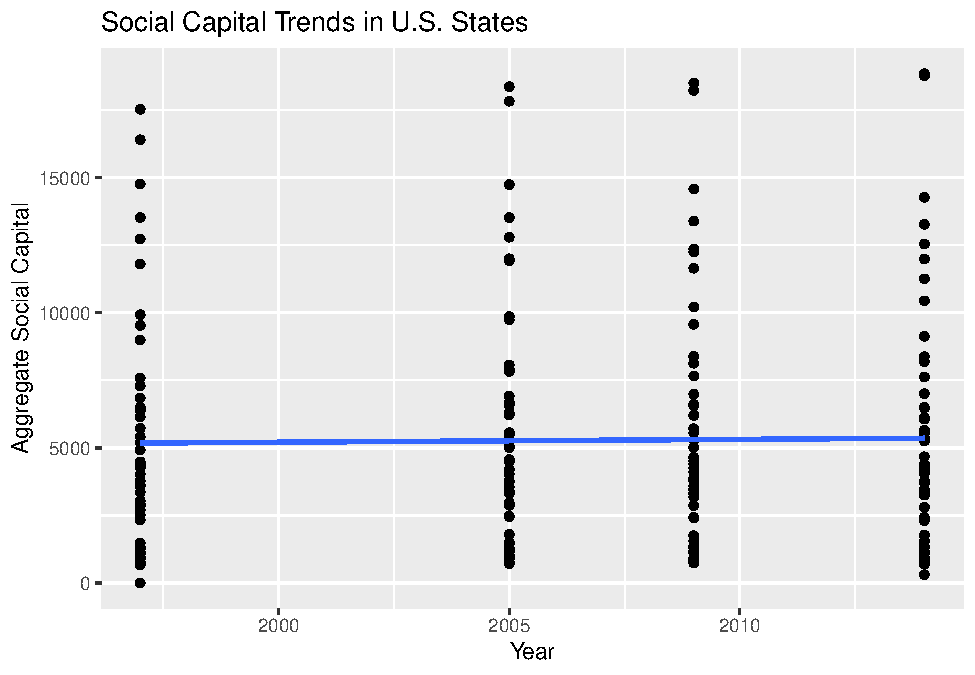
\includegraphics{Script_files/figure-latex/unnamed-chunk-1-1.pdf} 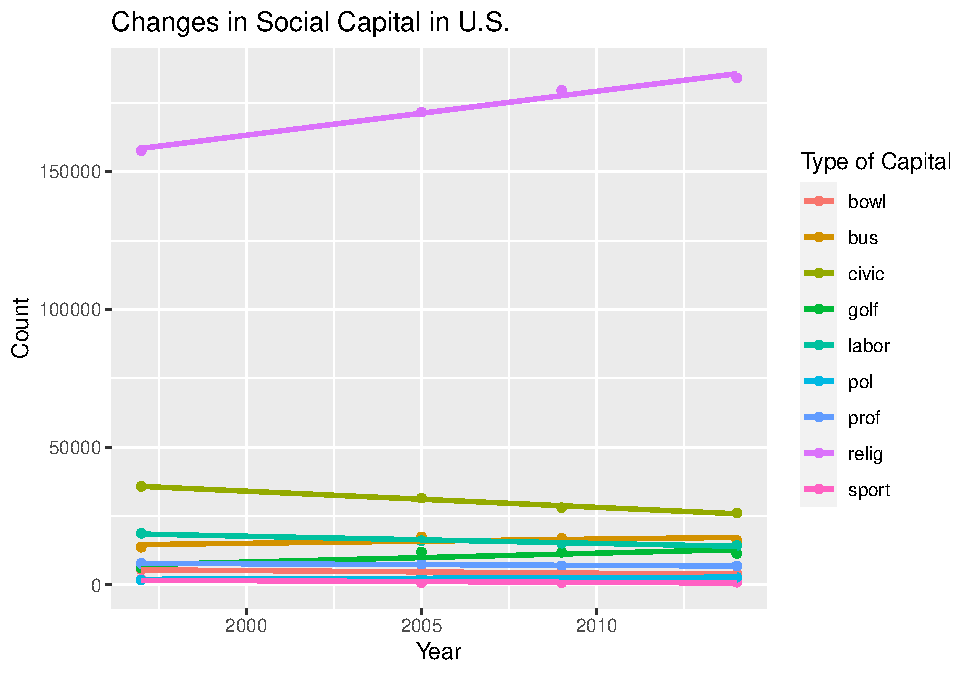
\includegraphics{Script_files/figure-latex/unnamed-chunk-1-2.pdf} 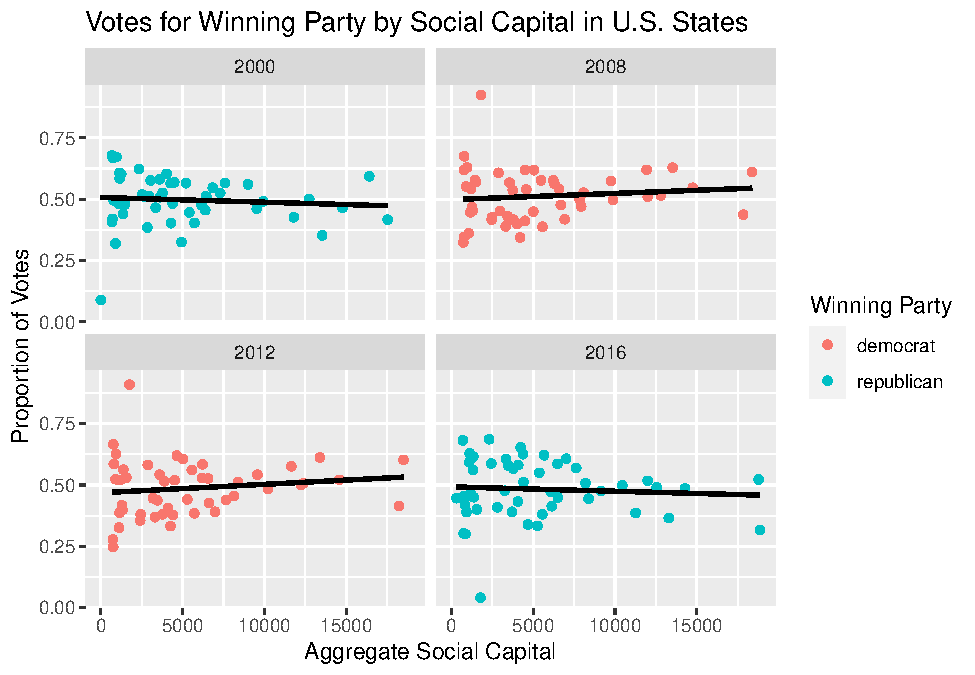
\includegraphics{Script_files/figure-latex/unnamed-chunk-1-3.pdf}

\begin{verbatim}
## Warning: package 'usmap' was built under R version 3.6.3
\end{verbatim}

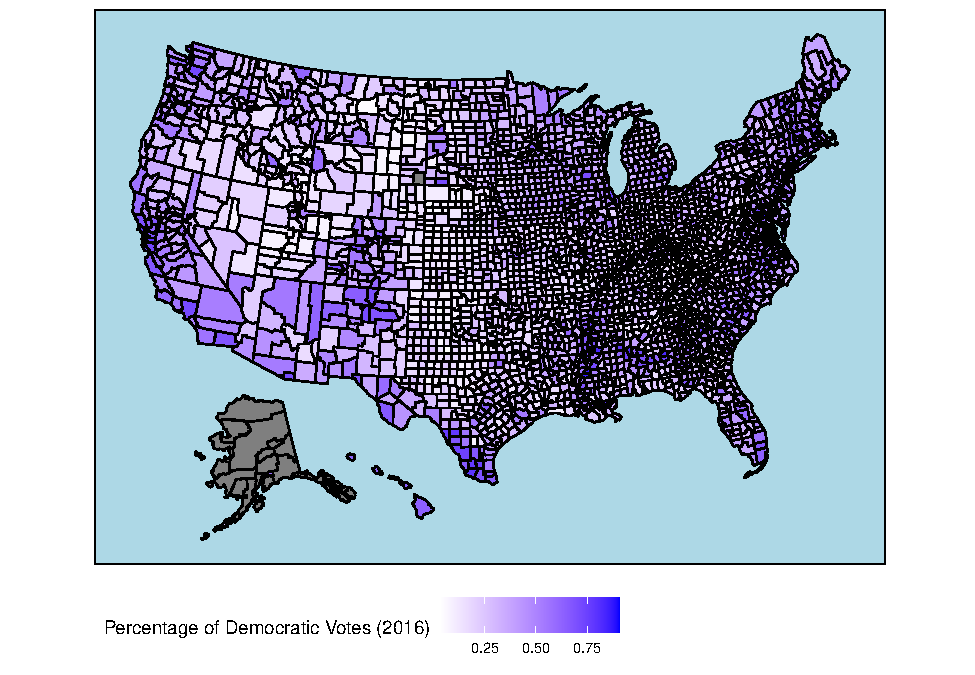
\includegraphics{Script_files/figure-latex/visualization part 2-1.pdf} 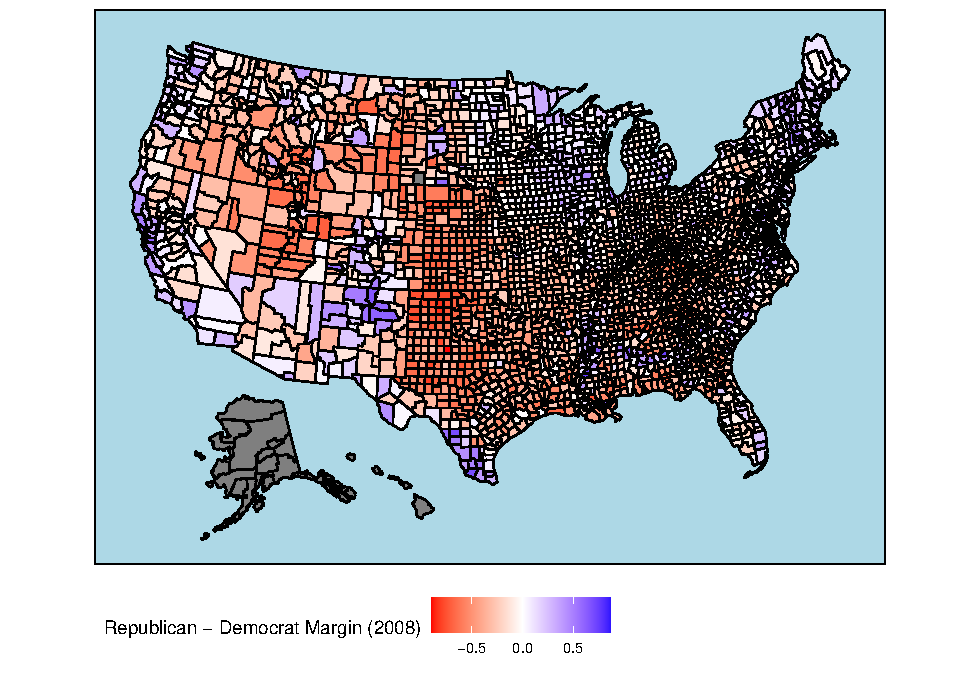
\includegraphics{Script_files/figure-latex/visualization part 2-2.pdf}

\begin{verbatim}
## [1] 2000 2008 2012 2016
\end{verbatim}

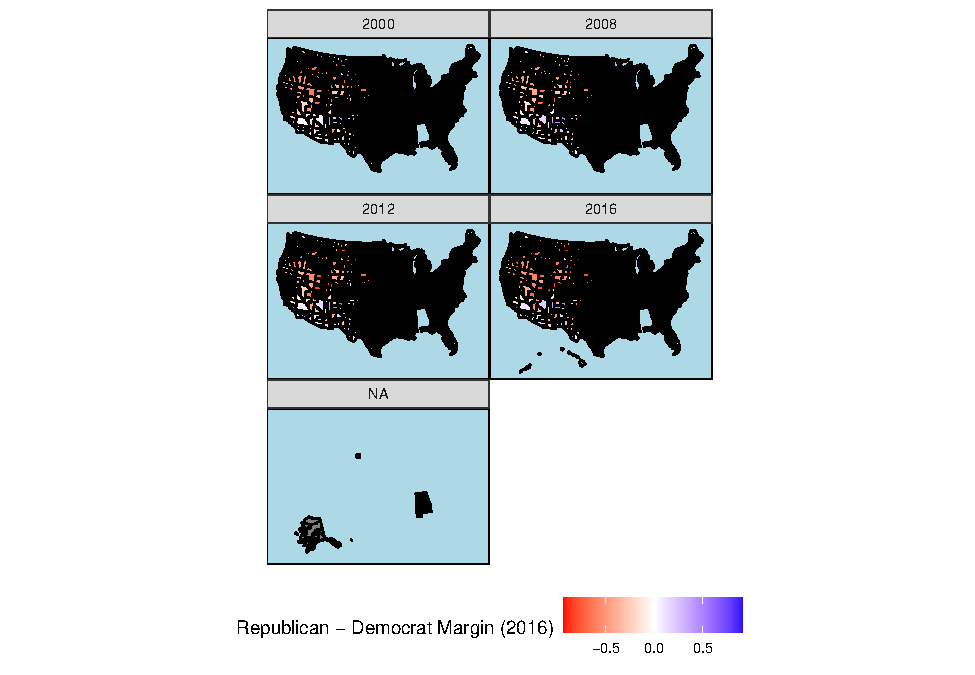
\includegraphics{Script_files/figure-latex/visualization part 2-3.pdf} 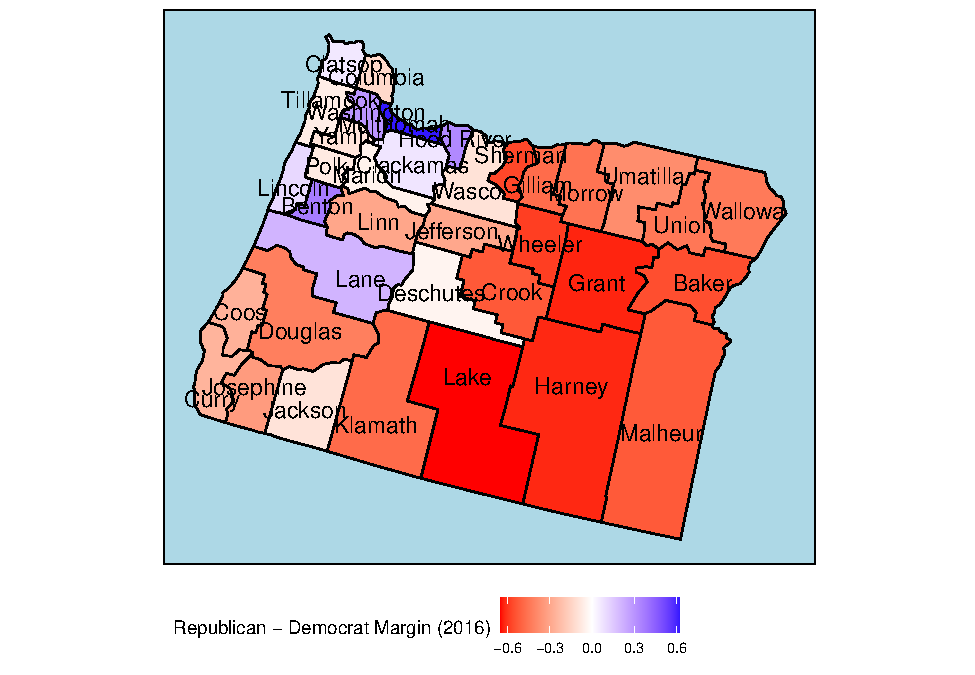
\includegraphics{Script_files/figure-latex/visualization part 2-4.pdf} 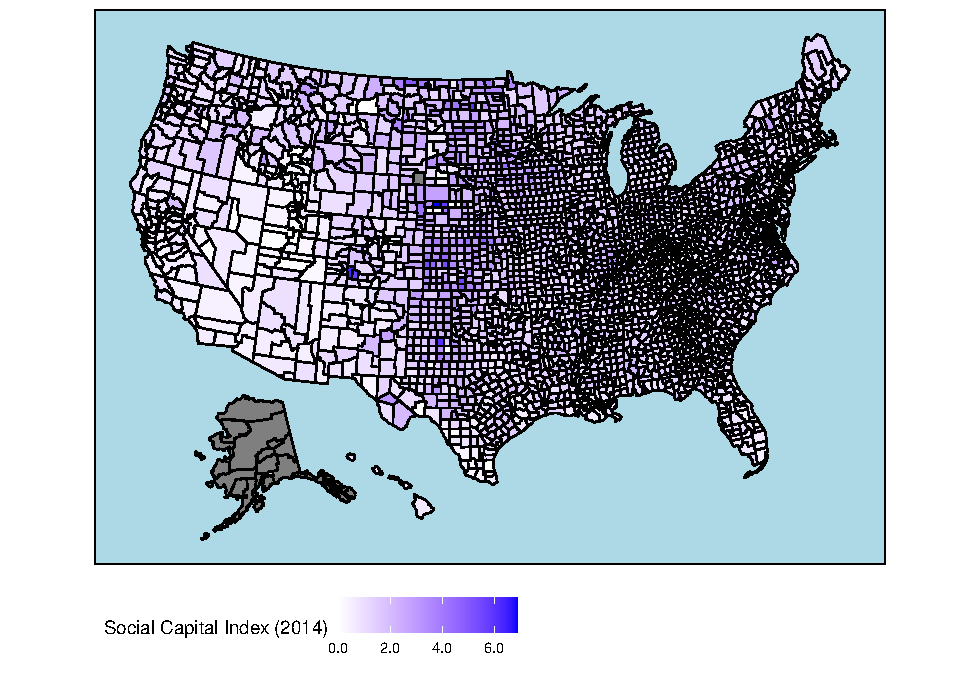
\includegraphics{Script_files/figure-latex/visualization part 2-5.pdf} 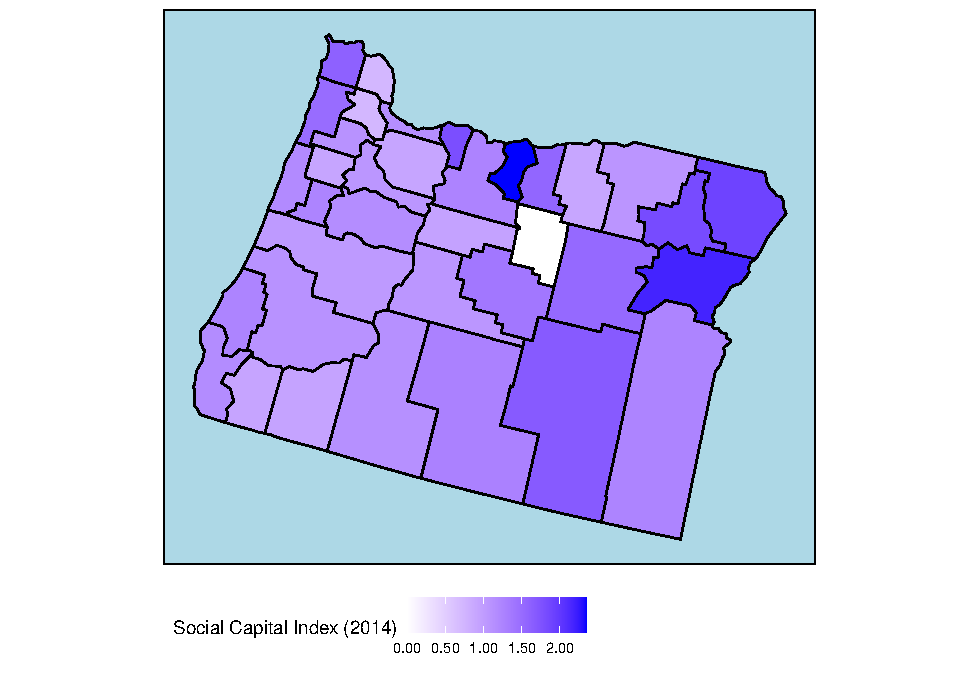
\includegraphics{Script_files/figure-latex/visualization part 2-6.pdf}

\hypertarget{results}{%
\section{Results}\label{results}}

\hypertarget{discussion}{%
\section{Discussion}\label{discussion}}

\newpage

\hypertarget{references}{%
\section{References}\label{references}}

\begingroup
\setlength{\parindent}{-0.5in}
\setlength{\leftskip}{0.5in}

\hypertarget{refs}{}
<<<<<<< Updated upstream
\leavevmode\hypertarget{ref-R-papaja}{}%
Aust, F., \& Barth, M. (2020). \emph{papaja: Create APA manuscripts with R Markdown}. Retrieved from \url{https://github.com/crsh/papaja}

\leavevmode\hypertarget{ref-R-magrittr}{}%
Bache, S. M., \& Wickham, H. (2014). \emph{Magrittr: A forward-pipe operator for r}. Retrieved from \url{https://CRAN.R-project.org/package=magrittr}

\leavevmode\hypertarget{ref-R-rio}{}%
Chan, C.-h., Chan, G. C., Leeper, T. J., \& Becker, J. (2018). \emph{Rio: A swiss-army knife for data file i/o}.

\leavevmode\hypertarget{ref-R-janitor}{}%
Firke, S. (2020). \emph{Janitor: Simple tools for examining and cleaning dirty data}. Retrieved from \url{https://CRAN.R-project.org/package=janitor}

\leavevmode\hypertarget{ref-R-purrr}{}%
Henry, L., \& Wickham, H. (2020). \emph{Purrr: Functional programming tools}. Retrieved from \url{https://CRAN.R-project.org/package=purrr}

\leavevmode\hypertarget{ref-R-here}{}%
Müller, K. (2017). \emph{Here: A simpler way to find your files}. Retrieved from \url{https://CRAN.R-project.org/package=here}

\leavevmode\hypertarget{ref-R-tibble}{}%
Müller, K., \& Wickham, H. (2020). \emph{Tibble: Simple data frames}. Retrieved from \url{https://CRAN.R-project.org/package=tibble}

\leavevmode\hypertarget{ref-R-base}{}%
R Core Team. (2020). \emph{R: A language and environment for statistical computing}. Vienna, Austria: R Foundation for Statistical Computing. Retrieved from \url{https://www.R-project.org/}
=======
\begin{CSLReferences}{0}{0}
\end{CSLReferences}
>>>>>>> Stashed changes

\leavevmode\hypertarget{ref-R-ggplot2}{}%
Wickham, H. (2016). \emph{Ggplot2: Elegant graphics for data analysis}. Springer-Verlag New York. Retrieved from \url{https://ggplot2.tidyverse.org}

\leavevmode\hypertarget{ref-R-stringr}{}%
Wickham, H. (2019). \emph{Stringr: Simple, consistent wrappers for common string operations}. Retrieved from \url{https://CRAN.R-project.org/package=stringr}

\leavevmode\hypertarget{ref-R-forcats}{}%
Wickham, H. (2020a). \emph{Forcats: Tools for working with categorical variables (factors)}. Retrieved from \url{https://CRAN.R-project.org/package=forcats}

\leavevmode\hypertarget{ref-R-tidyr}{}%
Wickham, H. (2020b). \emph{Tidyr: Tidy messy data}. Retrieved from \url{https://CRAN.R-project.org/package=tidyr}

\leavevmode\hypertarget{ref-R-tidyverse}{}%
Wickham, H., Averick, M., Bryan, J., Chang, W., McGowan, L. D., François, R., \ldots{} Yutani, H. (2019). Welcome to the tidyverse. \emph{Journal of Open Source Software}, \emph{4}(43), 1686. \url{https://doi.org/10.21105/joss.01686}

\leavevmode\hypertarget{ref-R-dplyr}{}%
Wickham, H., François, R., Henry, L., \& Müller, K. (2020). \emph{Dplyr: A grammar of data manipulation}. Retrieved from \url{https://CRAN.R-project.org/package=dplyr}

\leavevmode\hypertarget{ref-R-readr}{}%
Wickham, H., Hester, J., \& Francois, R. (2018). \emph{Readr: Read rectangular text data}. Retrieved from \url{https://CRAN.R-project.org/package=readr}

\leavevmode\hypertarget{ref-R-knitr}{}%
Xie, Y. (2015). \emph{Dynamic documents with R and knitr} (2nd ed.). Boca Raton, Florida: Chapman; Hall/CRC. Retrieved from \url{https://yihui.org/knitr/}

\endgroup


\printbibliography

\end{document}
